\documentclass[a4paper,12pt]{article} 
\usepackage[T2A]{fontenc}			
\usepackage[utf8]{inputenc}			
\usepackage[english,russian]{babel}
\usepackage{float}
\usepackage{amsmath,amsfonts,amssymb,amsthm,mathrsfs,mathtools} 
\usepackage{cancel}
\usepackage{multirow}
\usepackage[colorlinks, linkcolor = blue]{hyperref}
\usepackage{upgreek}\usepackage[left=2cm,right=2cm,top=2cm,bottom=3cm,bindingoffset=0cm]{geometry}
\usepackage{tikz}
\usepackage{graphicx}
\usepackage{subfig}
\usepackage{titletoc}
\usepackage{pgfplots}
\usepackage{xcolor}
\usepackage{wrapfig}
\usepackage{pgfplots}
\pgfplotsset{width=10cm,compat=1.9}

\begin{document}

\begin{titlepage}
		\vspace*{\fill}
		
		\begin{center}
			\includegraphics[scale=0.8]{MIPT.pdf}
			\\[0.7cm]\Huge Московский Физико-Технический Институт
			\\[2cm]\LARGE Отчет по эксперименту
			\\[0.5cm]\noindent\rule{\textwidth}{1pt}
			\\\Huge\textbf{4.4.3. \\ Изучение призмы с помощью гониометра}
			\\[-0.5cm]\noindent\rule{\textwidth}{1pt}
		\end{center}
		
		\vspace*{\fill}
		
		\begin{flushleft}
			Выполнила: \hspace{\fill} Группа:
			\\Малиновская София \hspace{\fill} Б05-102
		\end{flushleft}
	\end{titlepage}

	\setcounter{page}{2}


\section*{Цель работы} 
Знакомство с работой гониометра, исследование дисперсии стеклянной призмы и определение характеристик призмы как спектрального прибора.


\section*{В работе используются}
Гониометр, ртутная лампа, призма, стеклянная плоскопараллельная пластинка, призменный уголковый отражатель.


\section*{Теоретическая сводка}
Гониометр используется для точного определения углов, а значит с его помощью можно точно определять показатели преломления и преломляющие угла призм и кристаллов, измерять длины волн спектральных линий и прочее. Например, показатель преломления удобно определять по углу наименьшего отклонения. При это показатель преломления определяется формулой

\begin{equation}
    n = \frac{\sin \frac{\alpha + \delta}{2}}{\sin \frac{\alpha}{2}},
\end{equation}

\noindent
где $\alpha$ -- преломляющий угол призмы, $\delta$ -- угол минимального отклонения, $n$ -- показатель преломления. \\
Если $n_F$ -- показатель преломления голубой линии водорода, $n_D$ -- показатель преломления желтого дублета натрия, $n_C$ -- показатель преломления красной линии водорода, то можно определить

\begin{equation}
    D = n_F - n_C
\end{equation}
\begin{equation}
    \nu = \frac{n_D - 1}{n_F - n_C}
\end{equation}

\noindent
Также можно оценить разрещающую способность призмы по дисперсионной кривой (графику зависимости $n$ от $\lambda$)

\begin{equation}
    R = \frac{\lambda}{\delta\lambda} = b \frac{dn}{d\lambda}
\end{equation}

\noindent
где $\delta\lambda$ -- минимальный интервал длин волн из криетрия Релея, $b$ -- размер основания призмы.

\section*{Ход работы}
\paragraph{Юстриовка гониометра} настроили зрительную трубу, предметный столик, коллиматор, входную щель, начало отсчета. В общем, настроили все, что смогли. При этом ноль отсчета углов составляет $193^\circ11'23''$. Установили призму.

\paragraph{Измерение преломляющего угла} для этого установим трубу последовательно перпегдикулярно обеим преломляющим гранями призмы, измерив углы, соответствующие этим положениям ($193^\circ11'23''$ и $76^\circ9'45''$). По ним можем определить преломляющий угол призмы $\alpha = 62^\circ58'22''$.

\paragraph{Минимальный угол отклонения} для этого снача найдем спектр, получаемый с помощью призмы. Затем настроим на него зрительную трубу и измерим минимум отклонения для каждой из спектральных линий. Результаты занесем в табл. 1.

\begin{table}[H]
    \centering
    \caption{Координаты спектральных линий}
    \begin{tabular}{|c|c|c|c|c|} \hline
         № & $K_1$ & $K_2$ & 1 & 2 \\ \hline
         $\delta$ & $139^\circ06'39''$ & $138^\circ26'07''$ & $137^\circ50'03''$ & $137^\circ48'06''$ \\ \hline
    \end{tabular}
    \begin{tabular}{|c|c|c|c|c|} \hline
         № & 3 & 4 & 5 & 6 \\ \hline
         $\delta$ & $137^\circ15'59''$ & $135^\circ58'19''$ & $133^\circ48'53''$ & $131^\circ48'53''$ \\ \hline
    \end{tabular}
\end{table}

\noindent
Пользуясь формулой (1), рассчитаем показатели преломления $n$ для всех значений угла из табл. 1. Результаты представлены в табл. 2.

\begin{table}[H]
    \centering
    \caption{Показатели преломления}
    \begin{tabular}{|c|c|c|c|c|c|c|c|c|} \hline
         № & $K_1$ & $K_2$ & 1 & 2 & 3 & 4 & 5 & 6 \\ \hline
         $\lambda$, нм & 690.7 & 623.4 & 579.1 & 577.0 & 546.1 & 491.6 & 435.8 & 404.7 \\ \hline
         $n$ & 1.6329 & 1.6388 & 1.6440 & 1.6443 & 1.6488 & 1.6597 & 1.6774 & 1.6932 \\ \hline
    \end{tabular}
\end{table}

\noindent
Погрешность измерения считаем за $0^\circ0'1''$. При этом погрешность измерений $n$ слишком мала, а потому не учитывется. \\
Теперь построим дисперсионную кривую (рис. 1). 

\begin{figure}[H]
    \centering
    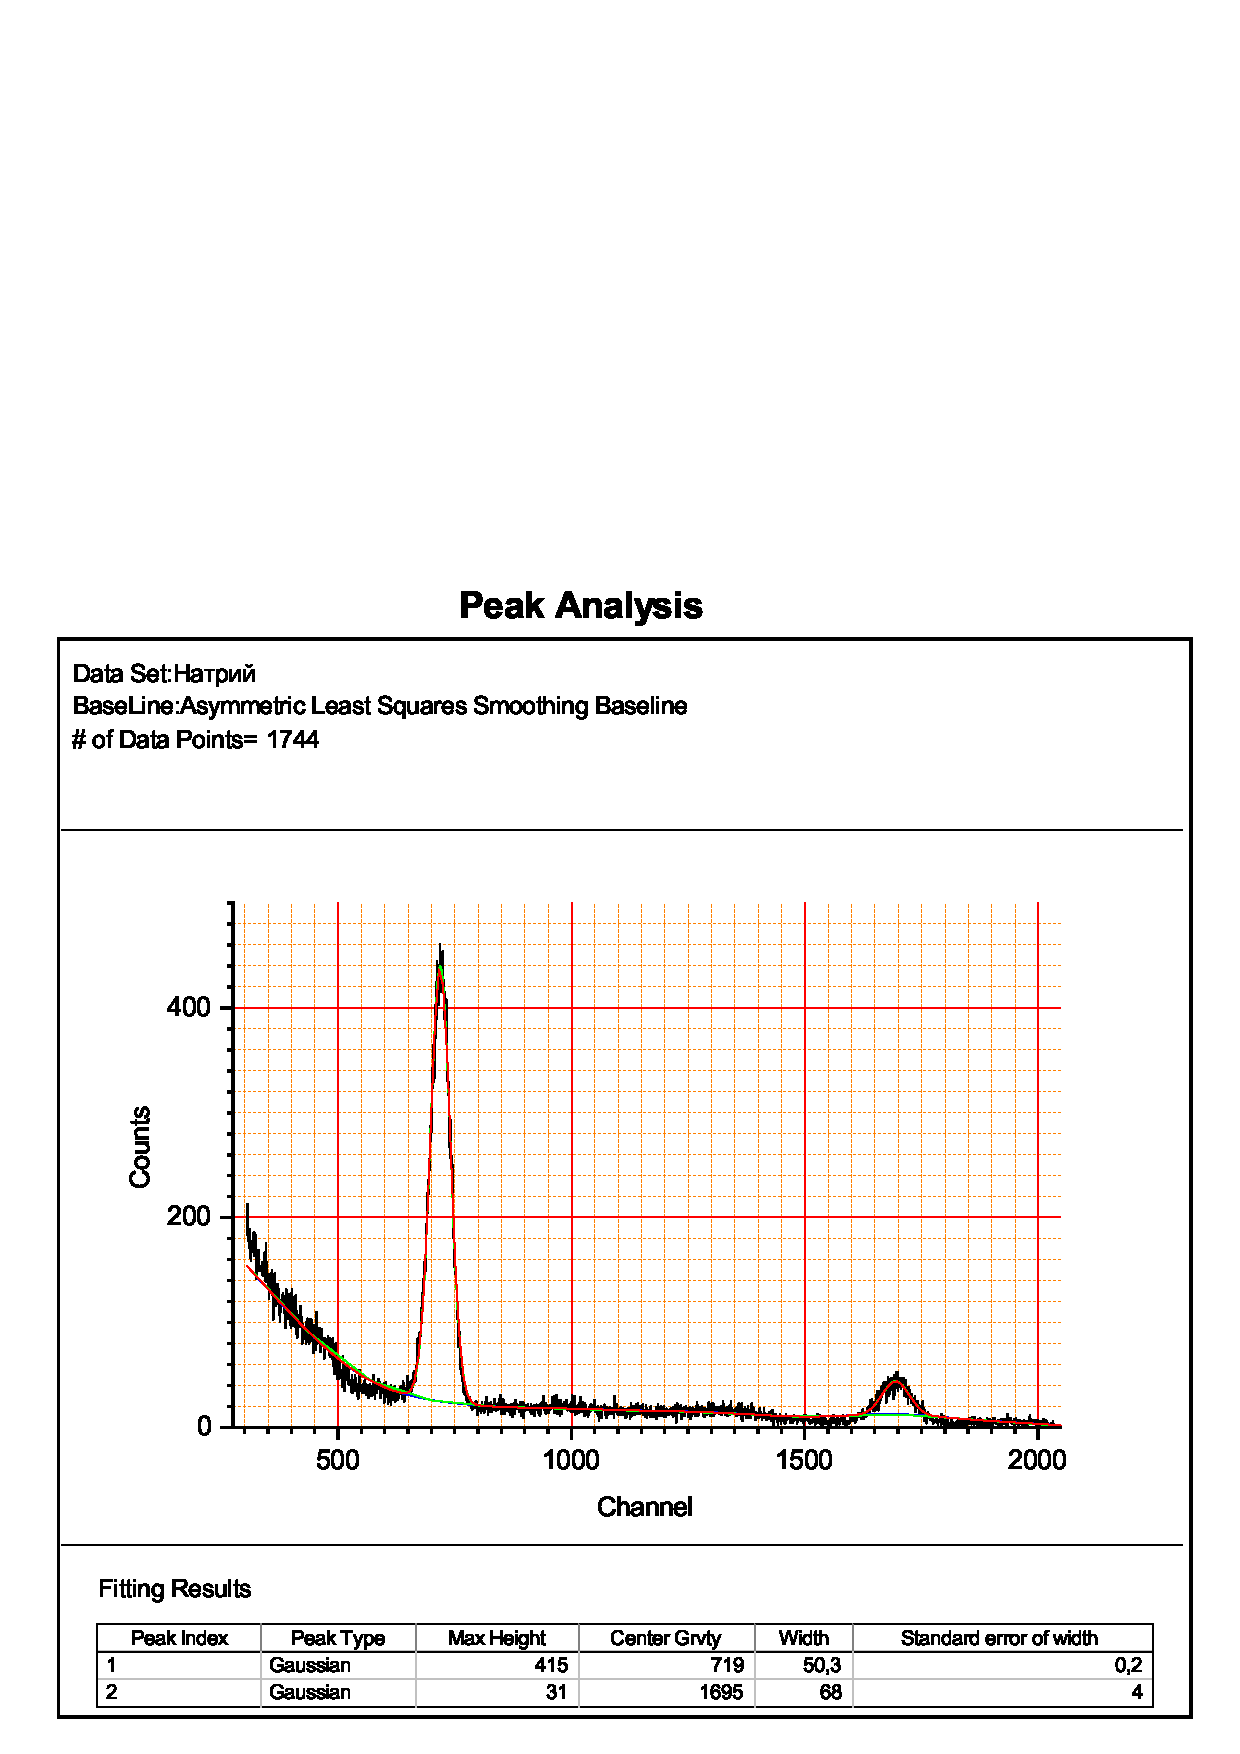
\includegraphics[scale=0.9]{1.png}
    \caption{Дисперсионная кривая}
\end{figure}

\noindent
Из графика получаем $n_D = 1.6428$, $n_F = 1.6614$, $n_C = 1.6359$. По формуле (2) находим $D = 0.0255$. По формуле (3) нахоим число Аббе $\nu = 28.5$. По этим параметрам можем предположить, что исследуемая призма сделана из тяжелого флинта (рис. 2).

\begin{figure}[H]
    \centering
    \includegraphics[scale=0.4]{abbe.png}
    \caption{Диаграмма Аббе для стекол[1]}
\end{figure}

\noindent
Длина основания призмы равна $b = 73$ мм. Из графика минимальное значение $\frac{dn}{d\lambda} = 8.767 \cdot 10^4$. Тогда по формуле (4) можем найти $R \approx 3400$. При этом $R \approx 300$, если считать по измерениям желтого дублета ($\delta \lambda = 20 \cdot 10^{-10}$ м). Отсюда реальный рабочий размер основания призмы составляет $3$ мм. Также определим угловую дисперсию по измерениям для желтого дублета $d\phi/d\lambda = 0.03 \; ^\circ/\text{нм}$.


\section*{Вывод}
Мы исследовали призму с использованием гониометра: 
\begin{itemize}
    \item посторили ее дисперсионную кривую (рис. 1)
    \item определили среднюю дисперсию $D = 0.0255$
    \item определили число Аббе $\nu = 28.5$
    \item определили характерные показатели преломления $n_D = 1.6428$, $n_F = 1.6614$, $n_C = 1.6359$
\end{itemize}
По этим данным определили, что скорее всего призма изготовлена из тяжелого флинта. \\
Также оценили разрешающую способность призмы $R \approx 300$ по желтому дублету и $R \approx 6300$ по углу наклона дисперсионной кривой. Отсюда сделали вывод, что реальный рабочий размер основания призмы значительно отличается от измеренного непосредственно. Также оценили угловую дисперсию призмы $d\phi/d\lambda = 0.03 \; ^\circ/\text{нм}$.


\begin{figure}[H]
    \centering
    \includegraphics[scale=0.2]{blue.png}
    \includegraphics[scale=0.2]{yellow.png}
    \includegraphics[scale=0.2]{red.png}
    \includegraphics[scale=0.2]{light_blue.png}
    \caption{Фотографии спектра ртутной лампы}
\end{figure}
\begin{figure}[H]
    \centering
    \includegraphics[scale=0.2]{purple.png}
    \caption{Фотографии спектра ртутной лампы}
\end{figure}


\section*{Литература}
\begin{enumerate}
    \item The Properties of Optical Glass. Schott Series on Glass and Glass Ceramics. 1998. ISBN 978-3-642-63349-2.
\end{enumerate}


\end{document}

